\newcommand{\neuron}[3]{
    \node[circle, draw=black, fill=#2] (#1) at #3 {};
}

\begin{frame}{Explainable artificial intelligence}
    \begin{tikzpicture}
        \node[] at (-5.25, -3.5) {};
        \node[] at (5.25, 3.5) {};

        \node[
            draw=black,
            fill=cyan!15,
            minimum height=3cm,
            minimum width=4.3cm,
            label=above:\footnotesize{\textbf{Artificial neural network}}
        ] (model) at (0, 0) {};

        \def\hsep{0.7}
        \def\vsep{0.5}
        \def\edgecolor{gray}
        \def\edgeopacity{0.5}
        \def\neuroncolour{gray}

        \only<1>{
            \neuron{n00}{\neuroncolour}{($ (model) + (-2 * \hsep, -2 * \vsep) $)}
            \neuron{n01}{\neuroncolour}{($ (model) + (-2 * \hsep, -\vsep) $)}
            \neuron{n02}{\neuroncolour}{($ (model) + (-2 * \hsep, 0) $)}
            \neuron{n03}{\neuroncolour}{($ (model) + (-2 * \hsep, \vsep) $)}
            \neuron{n04}{\neuroncolour}{($ (model) + (-2 * \hsep, 2 * \vsep) $)}

            \neuron{n10}{\neuroncolour}{($ (model) + (-\hsep, -1.5 * \vsep) $)}
            \neuron{n11}{\neuroncolour}{($ (model) + (-\hsep, -0.5 * \vsep) $)}
            \neuron{n12}{\neuroncolour}{($ (model) + (-\hsep, 0.5 * \vsep) $)}
            \neuron{n13}{\neuroncolour}{($ (model) + (-\hsep, 1.5 * \vsep) $)}

            \neuron{n20}{\neuroncolour}{($ (model) + (0, -\vsep) $)}
            \neuron{n21}{\neuroncolour}{(model)}
            \neuron{n22}{\neuroncolour}{($ (model) + (0, \vsep) $)}

            \neuron{n30}{\neuroncolour}{($ (model) + (\hsep, -0.5 * \vsep) $)}
            \neuron{n31}{\neuroncolour}{($ (model) + (\hsep, 0.5 * \vsep) $)}

            \neuron{n40}{\neuroncolour}{($ (model) + (2 * \hsep, 0) $)}

            \draw[-stealth, \edgecolor, opacity=\edgeopacity] (model.west) -- (n00);
            \draw[-stealth, \edgecolor, opacity=\edgeopacity] (model.west) -- (n01);
            \draw[-stealth, \edgecolor, opacity=\edgeopacity] (model.west) -- (n02);
            \draw[-stealth, \edgecolor, opacity=\edgeopacity] (model.west) -- (n03);
            \draw[-stealth, \edgecolor, opacity=\edgeopacity] (model.west) -- (n04);

            \foreach \i in {0,...,4} {
                \foreach \j in {0,...,3} {
                    \draw[\edgecolor, opacity=\edgeopacity] (n0\i) -- (n1\j);
                }
            }
            \foreach \i in {0,...,3} {
                \foreach \j in {0,...,2} {
                    \draw[\edgecolor, opacity=\edgeopacity] (n1\i) -- (n2\j);
                }
            }
            \foreach \i in {0,...,2} {
                \foreach \j in {0,...,1} {
                    \draw[\edgecolor, opacity=\edgeopacity] (n2\i) -- (n3\j);
                }
            }
            \foreach \i in {0,...,1} {
                \draw[\edgecolor, opacity=\edgeopacity] (n3\i) -- (n40);
            }

            \draw[-stealth, \edgecolor, opacity=\edgeopacity] (n40) -- (model.east);
        }
        \only<2>{
            \neuron{n00}{black!25}{($ (model) + (-2 * \hsep, -2 * \vsep) $)}
            \neuron{n01}{black!90}{($ (model) + (-2 * \hsep, -\vsep) $)}
            \neuron{n02}{black!72}{($ (model) + (-2 * \hsep, 0) $)}
            \neuron{n03}{black!99}{($ (model) + (-2 * \hsep, \vsep) $)}
            \neuron{n04}{black!10}{($ (model) + (-2 * \hsep, 2 * \vsep) $)}

            \neuron{n10}{black!55}{($ (model) + (-\hsep, -1.5 * \vsep) $)}
            \neuron{n11}{black!92}{($ (model) + (-\hsep, -0.5 * \vsep) $)}
            \neuron{n12}{black!31}{($ (model) + (-\hsep, 0.5 * \vsep) $)}
            \neuron{n13}{black!7}{($ (model) + (-\hsep, 1.5 * \vsep) $)}

            \neuron{n20}{black!50}{($ (model) + (0, -\vsep) $)}
            \neuron{n21}{black!10}{(model)}
            \neuron{n22}{black!100}{($ (model) + (0, \vsep) $)}

            \neuron{n30}{black!75}{($ (model) + (\hsep, -0.5 * \vsep) $)}
            \neuron{n31}{black!65}{($ (model) + (\hsep, 0.5 * \vsep) $)}

            \neuron{n40}{black!95}{($ (model) + (2 * \hsep, 0) $)}

            \draw[-stealth, \edgecolor, opacity=\edgeopacity] (model.west) -- (n00);
            \draw[-stealth, \edgecolor, opacity=\edgeopacity] (model.west) -- (n01);
            \draw[-stealth, \edgecolor, opacity=\edgeopacity] (model.west) -- (n02);
            \draw[-stealth, \edgecolor, opacity=\edgeopacity] (model.west) -- (n03);
            \draw[-stealth, \edgecolor, opacity=\edgeopacity] (model.west) -- (n04);

            \foreach \i in {0,...,4} {
                \foreach \j in {0,...,3} {
                    \draw[\edgecolor, opacity=\edgeopacity] (n0\i) -- (n1\j);
                }
            }
            \foreach \i in {0,...,3} {
                \foreach \j in {0,...,2} {
                    \draw[\edgecolor, opacity=\edgeopacity] (n1\i) -- (n2\j);
                }
            }
            \foreach \i in {0,...,2} {
                \foreach \j in {0,...,1} {
                    \draw[\edgecolor, opacity=\edgeopacity] (n2\i) -- (n3\j);
                }
            }
            \foreach \i in {0,...,1} {
                \draw[\edgecolor, opacity=\edgeopacity] (n3\i) -- (n40);
            }

            \draw[-stealth, \edgecolor, opacity=\edgeopacity] (n40) -- (model.east);

            \node[anchor=east, draw=black, inner sep=0pt] (input) at ($ (model.west) + (-0.77, 0) $) {
                
\includegraphics[width=2cm]{data/ladybug.png}
            };
            \cnnarrow{(input.east)}{(model.west)}{black}

            \node[anchor=west] (output) at ($ (model.east) + (0.77, 0) $) {
                Ladybug
            };
            \cnnarrow{(model.east)}{(output.west)}{black}
        }
        \only<3>{
            \neuron{n00}{red!25!black}{($ (model) + (-2 * \hsep, -2 * \vsep) $)}
            \neuron{n01}{red!90!black}{($ (model) + (-2 * \hsep, -\vsep) $)}
            \neuron{n02}{yellow!15!red}{($ (model) + (-2 * \hsep, 0) $)}
            \neuron{n03}{red!99!black}{($ (model) + (-2 * \hsep, \vsep) $)}
            \neuron{n04}{red!10!black}{($ (model) + (-2 * \hsep, 2 * \vsep) $)}

            \neuron{n10}{red!55!black}{($ (model) + (-\hsep, -1.5 * \vsep) $)}
            \neuron{n11}{yellow!20!red}{($ (model) + (-\hsep, -0.5 * \vsep) $)}
            \neuron{n12}{yellow!90!red}{($ (model) + (-\hsep, 0.5 * \vsep) $)}
            \neuron{n13}{red!7!black}{($ (model) + (-\hsep, 1.5 * \vsep) $)}

            \neuron{n20}{red!90!black}{($ (model) + (0, -\vsep) $)}
            \neuron{n21}{red!30!black}{(model)}
            \neuron{n22}{yellow!70!red}{($ (model) + (0, \vsep) $)}

            \neuron{n30}{yellow!40!red}{($ (model) + (\hsep, -0.5 * \vsep) $)}
            \neuron{n31}{red!65!black}{($ (model) + (\hsep, 0.5 * \vsep) $)}

            \neuron{n40}{red}{($ (model) + (2 * \hsep, 0) $)}

            \draw[stealth-, red, opacity=\edgeopacity] (model.west) -- (n00);
            \draw[stealth-, red, opacity=\edgeopacity] (model.west) -- (n01);
            \draw[stealth-, red, opacity=\edgeopacity] (model.west) -- (n02);
            \draw[stealth-, red, opacity=\edgeopacity] (model.west) -- (n03);
            \draw[stealth-, red, opacity=\edgeopacity] (model.west) -- (n04);

            \foreach \i in {0,...,4} {
                \foreach \j in {0,...,3} {
                    \draw[red, opacity=\edgeopacity] (n0\i) -- (n1\j);
                }
            }
            \foreach \i in {0,...,3} {
                \foreach \j in {0,...,2} {
                    \draw[red, opacity=\edgeopacity] (n1\i) -- (n2\j);
                }
            }
            \foreach \i in {0,...,2} {
                \foreach \j in {0,...,1} {
                    \draw[red, opacity=\edgeopacity] (n2\i) -- (n3\j);
                }
            }
            \foreach \i in {0,...,1} {
                \draw[red, opacity=\edgeopacity] (n3\i) -- (n40);
            }

            \draw[stealth-, red, opacity=\edgeopacity] (n40) -- (model.east);

            \node[anchor=east, draw=black, inner sep=0pt] (input) at ($ (model.west) + (-0.77, 0) $) {
                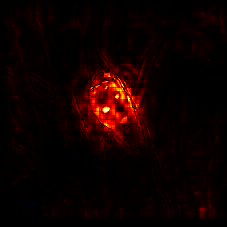
\includegraphics[width=2cm]{data/ladybug_explanation.png}
            };
            \lrparrow{(model.west)}{(input.east)}{red}

            \node[anchor=west, text=red] (output) at ($ (model.east) + (0.77, 0) $) {
                Ladybug
            };
            \lrparrow{(output.west)}{(model.east)}{red}
        }
    \end{tikzpicture}
\end{frame}